%
% Tallinn University of Technology - bachelor, master thesis template for LaTeX
%
% Public Version 1.1
% 2019 Adjusted by Frank Korving for his Bachelor Thesis, with contributions from Sander Arnus
%
% Public version 1.0
% 2010 - 2013 Thijs Nugteren and Joos Buijs for Master Thesis
%
% THIS IS THE MAIN FILE (i.e. compile this file, compiling the others directly won't work)
%
\documentclass[12pt, a4paper]{report}

% all the other includes etc. are done in the thesis.sty file.
\usepackage{thesis}

%
% These commands need to be defined in order to produce a correct and personalized document
%
\newcommand{\doctitle}{Polar spordikella andmeliides}
\newcommand{\docsubtitle}{bakalaureusetöö}

\newcommand{\me}{Rainer Liis}
\newcommand{\studentcode}{164039IACB}
\newcommand{\university}{TALLINNA TEHNIKAÜLIKOOL}
\newcommand{\school}{Infotehnoloogia teaduskond}
\newcommand{\department}{Arvutisüsteemide instituut}

\newcommand{\supervisor}{Jürgen Soom}
\newcommand{\supervisortitle}{}
\newcommand{\keywords}{Important, comma, separated, keywords, applicable, to, your, thesis}
\newcommand{\version}{0.1 version}
\newcommand{\monthYear}{Detsember 2020}
\newcommand{\Year}{2020}
\newcommand{\signatureDate}{Month Day, Year}

\author{\me}

%
% PDF settings
%
\hypersetup
{
    pdfauthor={\me},
    pdfsubject={\doctitle},
    pdfkeywords={\keywords}
}

\begin{document}
\pagenumbering{roman}
\begin{titlepage}
\headheight = 57pt
\footskip = 5pt
\headsep = 0pt

\centering
\textsc{\begin{Large}
\university\\
\end{Large} }
\school\\
\department\\

\vspace*{7 cm}

\begin{center}

\me \quad \studentcode\\
\begin{Large}
\textsc{\textbf{\doctitle}}\\
\end{Large}
\docsubtitle\\
\end{center}

\begin{flushright}
\textbf{Juhendaja: } \supervisor\\\supervisortitle\\
\end{flushright}

\vfill

Tallinn \Year
\end{titlepage}


\normalsize

\chapter*{\centerline{Autorideklaratsioon}}\label{chapter:declaration}
\hfill \\
Kinnitan, et olen koostanud antud lõputöö iseseisvalt ning seda ei ole kellegi teise poolt varem kaitsmisele esitatud.
Kõik töö koostamisel kasutatud teiste autorite tööd, olulised seisukohad, kirjandusallikatest ja mujalt pärinevad andmed on töös viidatud.

\vskip1in
\begin{flushleft}
\begin{tabular}{p{2.0cm}p{6.0cm}p{4.0cm}}
  Autor: & \me\\
  && \hfill\\
  Date: & \signatureDate &\\
  \\
  \\

% Uncomment the following to add supervisor declaration
%  \multicolumn{3}{l}{The thesis adheres to all specified requirements}\\
%  \hfill \\
%  Supervisor: & \supervisor & ......................................\\
%  && \hfill(signature)\\
%  Date: & \signatureDate &\\


\end{tabular}
\end{flushleft}


\chapter*{\centerline{Annotatsioon}}\label{chapter:abstract-eesti}


Lõputöö on kirjutatud ... keeles ning sisaldab teksti ... leheküljel, ... peatükki, ... joonist, ... tabelit.

\pagebreak

\chapter*{\centerline{Abstract}}\label{chapter:abstract}
The thesis is in ... and contains ... pages of text, ... chapters, ... figures, ... tables.
\pagebreak

\chapter*{\centerline{Lühendite ja mõistete sõnastik}}\label{chapter:terms}
\begin{longtable}{p{3cm}p{10cm}}
API&\textit{Application Programming interface} ehk Rakendusliides\\
HID&\textit{Human Interface Device} ehk Inimliidesega seade\\
IO&\textit{Input and Output} ehk sisend ja väljund\\
USB&\textit{Universal Serial Bus} ehk Universaalne andmeliides\\
\end{longtable}
\addtocounter{table}{-1} 

\pagebreak

\phantomsection
\setcounter{tocdepth}{2}    % Sets maximum depth of Table Of Contents
\renewcommand{\contentsname}{Sisukord}
\tableofcontents

\clearpage \phantomsection
\setcounter{figure}{0}
\addcontentsline{toc}{chapter}{\listfigurename}
\listoffigures

\clearpage \phantomsection
\addcontentsline{toc}{chapter}{\listtablename}
\listoftables

\chapter{Sissejuhatus}\label{chapter:introduction}
\onehalfspacing
\setcounter{page}{0}
\pagenumbering{arabic}   %from here on, start the 'real' page numbering, from 1, with normal digits
%%Some basic ways to manipulate text are \textit{italics} and \textbf{bold}. One can reference Figures (see Figure \ref{fig:taltech} for an example) as well as cite references which are defined in the \textit{references.bib} file.\cite{spectre,example-reference} 
%The \textit{Bibliography}, \textit{List of Figures} and \textit{List of Tables} are all automatically generated and references will be updated automatically as well. This means that if you've defined a citation but are not referencing it, it will not appear in the \textit{Bibliography}. This also means that any Figure / Table / Citations numbers are automatically updated as well. Numbering is done by order-of-appearance.
%
%One can create an itemized list:
%\begin{itemize}
%    \item item a
%    \item item b
%    \item ...
%\end{itemize}
%
%Or enumerate them:
%\begin{enumerate}
%    \item item x
%    \item item y
%    \item ...
%\end{enumerate}
%
%
%\begin{figure}[ht]
%    \centering
%    
\includegraphics[width=.5\textwidth]{figures/taltech.jpg}
%    \caption{\textit{An image of the TalTech logo.}}
%    \label{fig:taltech}
%\end{figure}
%
%
%A table with three columns can be seen in Table \ref{tab:requirements}.
%\begin{longtable}{|p{0,5cm}|p{10cm}|p{3cm}|}
%	\caption{\it{A table with some requirements}}
%	\label{tab:requirements}\\ \hline
%	\textbf{Nr} &  \textbf{Requirement} & \textbf{Weight}  \\
%	\hline
%	\endfirsthead
%	\multicolumn{3}{l}%
%	{\tablename\ \thetable\ -- \textit{Continues...}} \\
%	\hline
%	\textbf{Nr} &  \textbf{Requirement} & \textbf{Importance}  \\
%	\hline
%	\endhead
%	\hline \multicolumn{3}{l}{\textit{Continues...}} \\
%	\endfoot
%	\hline
%	\endlastfoot
%1 & Price & High\\ \hline
%2 & Variety& Middle\\ \hline
%3 & Support& Low\\ \hline
%
%%%\end{longtable}
%%
%We can use variables set in the \textit{main.tex} file to render values like our title (\doctitle) or supervisor names (\textbf{Supervisor}: \supervisor, \textbf{Co-supervisor}: \cosupervisor{}).

Lõputöö eesmärgiks oli luua programm, mis liidestub Polar RC3 GPS spordikellaga ning pärib sealt andmeid, mida siis kasutajale vormistatult väljastada. 
Spordikell liidestub arvutiga USB kaudu saades arvutilt päringuid, millele siis vastatakse.\cite{example-reference}


\chapter{Kella tutvustus}\label{chapter:first_chapter}
%This is the first real chapter of this thesis. Other chapters can be easily referenced, for example the introduction can be found as Chapter \ref{chapter:introduction}. Sections and/or subsections need to be labeled before one can reference them. See Section \ref{sec:second-section} for an example.

%\section{First Section of the First Chapter}
%Some text in the first section.
%\subsection{First Subsection}
%As well as some text in this subsection.
%\subsubsection{First Subsubsection}
%The Table of Contents only goes 3 layers deep (Chapter - Section - Subsection) so this subsubsection is not seen there.

%\section{Second Section of the First Chapter}\label{sec:second-section}

Projektis kasutatud spordikell on Polar RC3 GPS.

Kellaga on kaasas ka manual, kus on välja toodud kella omadused.\cite{rc3-man}
Konkreetne mudel on toodetud aastal 2013.

\section{Kella riistvara}\label{sec:riistvara}
\begin{figure}[ht]
    \centering
    \includegraphics[width=.5\textwidth]{figures/watch.jpg}
    \caption{\textit{Pilt kella emalplaadist}}
    \label{fig:watch}
\end{figure}

Projekti alguses tutvuti ka kella riistvaraga, võttes kell lahti ja uurides selle komponente.
Kuna kella pidi saama ka hiljem kasutada, ei hakatud antud projekti käigus lahti võtma kella komponente, et neid lähemalt uurida.
Kella riistvara kohta avalikku dokumentatsiooni ei leitud ning kella enda emaplaati uurides ka ei olnud lihtne aru saada, millised konkreetsed detailid sellel olid.
Kella uuriti mikroskoobi all ning iga komponendi kohta pandi kirja kõik informatsioon, mis oli võimalik leida.
Hiljem internetist nende komponentide kohta informatsiooni otsimine ei andnud tulemusi, kuna ei olnud võimalik piisavalt täpselt otsida.

\section{Tootjapoolne tarkvara}\label{sec:tootja-soft}
Polari tarkvara, millega sai kellast andmeid tõmmata ja analüüsida, oli Polar WebSync.
Selle tööpõhimõte oli järgnev:
Tuli ühendada kell arvuti külge, seejärel käivitada rakendus.
Andmete kättesaamiseks ja vaatamiseks oli vaja luua kasutajakonto nende veebikeskkonda.
Kui konto oli olemas, tuli logida sisse enda kasutajanime ja parooliga rakendusse, mis seejärel tõmbas andmed kellast pilve, kus neid siis töödeldi ja seejärel sai andmeid veebilehitsejas sisselogituna vaadata. 
Kasutaja masinasse andmeid ei jäetud, nii et neist koopiat teha ei olnud võimalik.
Aasta 2019 lõpus\cite{polar-ws-discontinued} lõpetati toetus ära rakendusele WebSync ja sulgeti ka veebikeskkond polarpersonaltrainer.com, kuna see oli vana ja sooviti keskenduda uue süsteemi toetamisele.
Uus keskkond on tehniliselt erinev vanast, nii et andmete üle toomine ning vana rakenduse kasutamine ei olnud võimalik.
Selle tagajärjel on inimesed, kes kasutavad vana riistvara jäänud ilma võimalusest oma treeningute andmeid analüüsida rohkem, kui kellast iga individuaalse treeningu andmeid vaadates.

Kell suhtleb arvutiga kasutades USB ühendust.

USB standard klassifitseerib ära seadmete klassid. Antud kell klassifitseerub HID seadmeks, mis tähendab seda, et see on seade millega inimesed saavad otseselt kasutada.
HID seadmete jaoks on ette nähtud omaette suhtlusviis, kuidas saab edastada teateid seadmele ja sealt infot kätte.

kirjelda kuidas see suhtlus on et koigepealt avad jne 

siis kuidas see muu osa seal on et ei taha seda surnuks pommitada

mis asjad on endpointid jne



\chapter{USB}\label{chapter:usb}
%One of the best resources for \LaTeX basics, and advanced constructs, is the \LaTeX wikibook\footnote{To be found at~\url{http://en.wikibooks.org/wiki/LaTeX/}}. Of course fellow students, colleagues and a good internet search using your favorite search engine can do wonders if you're stuck. 

\section{Libusb}\label{sec:libusb}
Libusb on universaalne teek, kirjutatud C keeles, et hõlbustada programmide loomist, mis suhtlevad USB seadmetega.

Kell suhtleb arvutiga kasutades USB ühendust.

USB standard klassifitseerib ära seadmete klassid. Antud kell klassifitseerub HID seadmeks, mis tähendab seda, et see on seade millega inimesed saavad otseselt kasutada.
HID seadmete jaoks on ette nähtud omaette suhtlusviis, kuidas saab edastada teateid seadmele ja sealt infot kätte.

kirjelda kuidas see suhtlus on et koigepealt avad jne 

siis kuidas see muu osa seal on et ei taha seda surnuks pommitada

mis asjad on endpointid jne



\chapter{Metoodikad}\label{chapter:metoodika}
Kellast andmete pärimine on teadmata protsess antud projekti raames.
Andmetele ligipääsu saamiseks on erinevaid metoodikaid, mida ka allpool kirjeldatatakse ja ka põhjendatakse, miks konkreetne valik tehti.

\section{Originaalse rakenduse jäljendamine}
Lihtsaim variant oleks ühendada kell arvuti külge, millel töötab tootja enda originaalne rakendus ning kasutada seda andmete kättesaamiseks, samal ajal USB liini jälgides.
USB liini jälgimiseks saab kasutada nii tarkvara, nt Wireshark, kui ka riistvaralist lahendust.
Kui on käes suhtlus kella ja arvuti vahel, saab saadud tulemust proovida jäljendada.
Sellise tegutsemise juures on ka oht kella kahjustada kõige väiksem, kuna seda peab vähem ebavajalike päringutega "pommitama".
Kuna originaaltarkvara töötas vaid Mac ja Windows keskkondades, on selleks vaja töötavat arvutit sellise operatsioonisüsteemiga.

\section{Sarnase projekti jäljendamine}
Keerukam lahendus on leida mõni sarnane projekt ja tutvuda sellega, kuidas antud programm töötab.
Kui leitud tarkvara toimib, saab proovida seda jäljendada.
Kui see ei toimi, tuleb seda proovida kohandada, et see tööle hakkaks.
Selline lähenemine hõlmab palju katsetamist, mis ei ole optimaalne.
Katsetamise kaks suuremat miinust on ajakulu ja ka võimalus, et saates kellale suvalisi päringuid, võib üle kirjutada kätte saada tahetavaid andmeid, kui ka suuremat kahju teha.

\section{Valitud metoodika}
Esimene valik projekti alustades oli originaalse rakenduse jäljendamise tee, kuna see tundus kõige lihtsam ja selgem viis probleemi lahendamiseks.
Selle proovimise käigus selgus, et nii konkreetse seadme toetus, kui ka serveripoolne teenus, mis võimaldas vaadata ja hoiustada andmeid on töötamise lõpetanud ja kasutajatele enam kättesaamatu.
Rakendus andmeid kasutaja seadmesse ei salvestanud, vaid suunas need otse pilve, mille tõttu ei olnud enam võimalik kasutada seda rakendust ka lihtsalt andmete saamise protsessi õppimise jaoks.




\chapter{Programmi töö kirjeldus}\label{chapter:kirjeldus}

\begin{figure}[ht!]
    \centering
    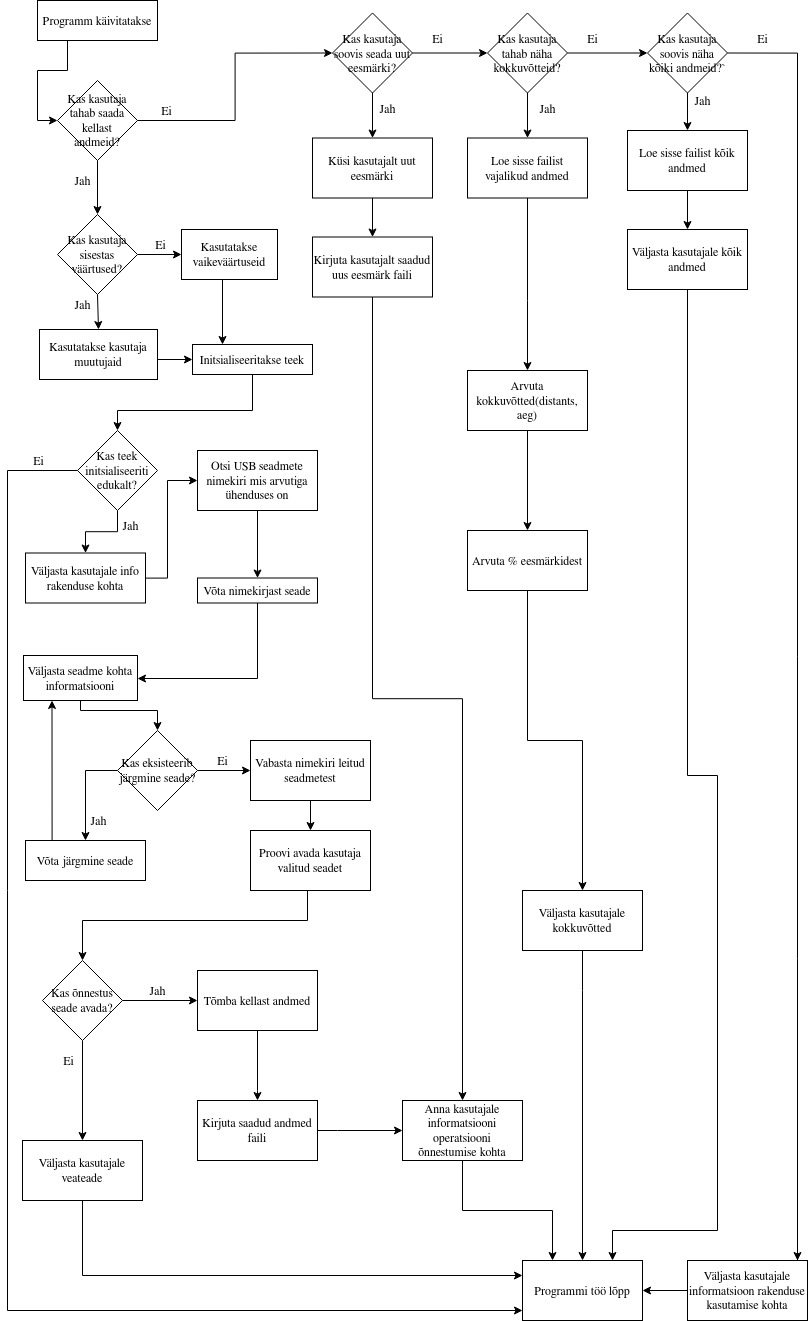
\includegraphics[width=.75\textwidth]{figures/flowchart.jpg}
    \caption{\textit{Voodiagramm programmi planeeritud tööst}}
    \label{fig:flowchart}
\end{figure}
\pagebreak

\section{Olemasoleva programmi töö}\label{sec:programmi-too}
Programmi alguses määratakse ära vaikeväärtused, mida rakendus saab kasutada.
Seejärel initsialiseeritakse \textit{libusb} teek ning antakse kasutajale teada mis versioon teegist kasutusel on.
Kui kasutaja on andnud rakendusele kaasa parameetrid, mille järgi soovib leida seadet, millega suhelda siis otsitakse seda konkreetset seadet ja kui kasutaja ei ole neid kaasa andnud, kastuatakse vaikeväärtuseid.
Kui otsitavat seadet ei leita, lõpetatakse programmi töö.
Kui otsitav seade on olemas ja ligipääsetav, siis programm jätkab seadme kohta informatsiooni väljastamisega.
Enne kellale päringute saatmist peab seadme avama, mida ka tehakse.
Kui avamine õnnestub, teatakse kasutajale, et see õnnestus, kui ei siis programmi töö katkestatakse.
Seejärel peaks hakkama kellast informatsiooni hankimine, kuid seda programmi osa projekti raames valmis ei saadud.

\section{Programmi fookus}\label{sec:arenduskaik}
Vaadates joonist~\ref{fig:flowchart} on näha, et kõige detailsemalt on kirjeldatud andmete hankimise osa ning rakenduse kasutajapoolne osa on lihtsam.
Rakenduse arenduse käigus otsustati, et proovitakse saada andmete saamise osa enne valmis, kui hakatakse kasutaja poolt valmistama.
Sellise valiku tingis võimalikkus 3 lõpptulemuse vahel.

Esimene neist oleks programm, mis suudab tõmmata kellast andmed ja on muus osas poolik.
Selline lahendus oli parim saavutatav tulemus, kuna sinna otsa kasutajaliides ehitada oleks olnud kiirem protsess ja see oli ühtlasi ka antud programmi kontekstis vähemtähtis.
Teine variant oleks olnud alustada kasutajaliidesega ja suunata see käsitsi kirjutatud faili lugema ja sealt andmeid võtma. 
Seda ei valitud kuna lõppeesmärgi saavutamiseks, mis oli siis kellast saadud andmete töötlemine, oleks pidanud topelt tööd tegema, kuna käsitsi kirjutatud fail poleks ilmselt olnud ühilduv kellast tulnud andmetega.  
Esimesega kaasaskäiv kõige halvem võimalik tulemus oli, et projekti lõpuks ei valmi ei andmete hankimise osa, kui ka kasutajaliides, nii et projekt jääb ilma töötava programmita.

Eelnevalt loetletud lõpptulemuste vahel valides vaadati, milline osa projektist kõige tähtsam on.
Kasutaja andmete analüüsimise koha pealt oleks tulnud just esimesena teha valmis kasutajaliides.
Projekti suurim eesmärk aga oli luua liides just Polar kellale, millega oleks kasutajatel ligipääs enda kogutud andmetele, millega siis edasi toimida.
Loetletud põhjused tingisidki vajaduse saada esimesena andmed kätte ja õigustasid riski projekt mitte valmis saada.

\chapter{Olemasoleva tarkvara võrdlus}\label{chapter:soft}

\section{Tootjapoolne tarkvara}\label{sec:tootja-soft}
Polari tarkvara, millega sai kellast andmeid tõmmata, oli Polar WebSync.
Selle tööpõhimõte oli järgnev:
Tuli ühendada kell arvuti külge, seejärel käivitada rakendus.
Andmete kättesaamiseks ja vaatamiseks oli vajalik kasutajakonto nende veebikeskkonnas.
Kui konto oli olemas, tuli logida sisse enda kasutajanime ja parooliga rakendusse, mis seejärel tõmbas andmed kellast veebikeskkonda polarpersonaltrainer.com, ilma kasutaja masinasse andmeid salvestamata, kus neid siis töödeldi ja seejärel sai andmeid veebilehitsejas sisselogituna vaadata. 
Aasta 2019 lõpus lõpetati toetus ära rakendusele WebSync ja sulgeti ka veebikeskkond, kuna see oli vana ja sooviti keskenduda uue süsteemi toetamisele.\cite{polar-ws-discontinued}

Uus keskkond on tehniliselt piisavalt erinev vanast, et andmete üle kandmine vanast keskkonnast polnud võimalik.
Vanemad seadmed ning vana rakendus uue keskkonnaga ei liidestu.
Vanemate seadmete omanikele pakuti üleminekuperioodil, mis lõppes 29. veebruar 2019, ka soodustusi uuema riistvara ostmiseks.\cite{polar-ws-discontinued}
Selle muudatuse tagajärjel on inimesed, kes kasutavad ikkagi vana riistvara, jäänud ilma võimalusest oma treeningute andmeid analüüsida rohkem, kui kellast iga individuaalse treeningu andmeid vaadates.

Sellel rakendusel oli mitu negatiivset omadust.
Suurim neist oli, et kasutaja ei omanud oma andmeid ja pidi kasutama tootja enda keskkonda enda andmete nägemiseks, kuhu ilma registreerimata ligi ei pääsenud.
Eelnevaga kaasaskäiv miinus on, et andmete nägemiseks oli vajalik internetiühendus, kuna kõik andmed elasid pilves.
Lisaks eelnevalt mainitud puudujääkidele ei olnud rakendus saadaval Linux platvormil, mis tähendab et osad kasutajad pidid leidma mingi viisi kasutada kas Windows või Mac platvormi.
Lisaks negatiivsetele omadustele oli ka positiivne, et rakendus töötas hästi ja oli kergelt arusaadav kasutajale.


\section{Polar-Flowlink-linux}\label{sec:flowlink}
Projekti tegemise poole peal leiti ka githubist analoogne projekt kunagise WebSync tarkvaraga.
Leitud tarkvara nimi on Polar flowlink.
Flowlink koosneb mitmest osast:
Esimene osa tõmbab kellast andmed, teine suunab need andmebaasi ning kolmas osa oli veebiliides, millega on võimalik saadud andmeid vaadata.
Projekti kirjelduses oli ka kirjas, et see rakendus on kirjutatud Polar FT60 HRM jaoks.
Autor ka väitis et proovis programmi FT80 mudeliga ja selle peal see ei töötanud.
Seda projekti prooviti ka autori kellaga ning sellega samamoodi ei saadud andmeid kätte.

Leitud projekti puhul on suur eelis, et lähtekood on avatud ja siis saab sellega tutvuda, et saada aimu sellest, kuidas see töötama peaks.
Miinustena saab välja tuua aga sobimatuse seadmega, mis ka muudab kogu rakenduse mittekasutatavaks.
Andmete saamisele lisaks töötavad andmebaas ja veebiliides on ka antud rakenduse jaoks üleliigsed.


\section{Võrdlus}
Mõlemal olemasoleval ja leitud rakendusel on nii positiivseid külgi kui ka negatiivseid.
Kui mõlemad töötaksid ja ühilduksid kellaga, saaks neid kasutada küll andmete visualiseerimiseks ja analüüsimiseks, kuid 
Kuigi tootja enda tarkvara oli palju rohkemate omaduste ja funktsionaalsustega, kui leitud analoog, oleks see siiski ebamugav lahendus liiga paljude osadega.
Eraldiseisvat rakendust on vaja, et oleks olemas ka äärmiselt lihtne ja minimaalne liides andmete nägemiseks.


\chapter{Kokkuvõte}\label{chapter:summary} 
Käesoleva lõputöö eesmärk oli luua lihtne ja minimaalne andmeliides Polar RC3 GPS spordikellale, mis suudaks sealt saada kätte kasutaja treeningandmed ja võimaldaks kasutajal siis neid analüüsida.

Projekti käigus prooviti tutvuda kella tööpõhimõttega ning sellele toetudes kirjutada tarkvara.
Kella riistvaraga tutvuti kell lahti võttes ja visuaalselt vaadeldes, komponente lahti emaplaadilt ei võetud.
Andmeedastust prooviti uurida kasutades olemasolevat tootjapoolset programmi.
Leitud alaoogset lahendust originaalsega prooviti kasutada ja ka kohandada soovitud tulemuse saavutamiseks, kuid lõplik lahendus oli sobiva tarkvara ise kirjutamine, mis jäi poolikuks.

Andmete kellast kättesaamine osutus liiga keeruliseks ja sellega seoses olid liiga suured takistused, mida selle projekti raames ei suudetud kõrvaldada.
Põhiliseks takistuseks osutus kellaga suhtlemiseks õige viisi leidmine, kuna dokumentatsioon puudus ja originaalne rakendus enam ei tööta.
Programm on valminud kuni seadme avamiseni ja andmeid seadmest kätte ei saa.

Tulevikus tuleks jätkata programmi arendamist, et saada kätte sobiv lahendus, mis võimaldaks kasutada täielikult ka vanemaid seadmeid, millele enam toetust tootja poolt pole.

\pagebreak
\phantomsection
\addcontentsline{toc}{chapter}{Kasutatud kirjandus}
\printbibliography

 %   \pagebreak
 %   \phantomsection
 %   \appendix
 %   \addcontentsline{toc}{chapter}{Appendices}
 %   \chapter*{Appendices}
 %   \renewcommand{\thechapter}{\arabic{chapter}}

 %  \addcontentsline{toc}{chapter}{Appendix 1 - Something}\label{chapter:appendix-one}
 %   {\let\clearpage\relax\chapter*{Appendix 1 - Something}}
 %   \begin{lstlisting}[frame=single, basicstyle=\small]
<!DOCTYPE html>
<html>
<body>

<h1>Example Title</h1>

<p>Some text here</p>

</body>
</html>
\end{lstlisting}

 %   \clearpage
 %   \phantomsection
 %   \addcontentsline{toc}{chapter}{Appendix 2 - Something Else}\label{chapter:appendix-something-else}
 %   \chapter*{Appendix 2 - Something Else}
 %   \textbf{Pythagorean theorem}
\begin{equation}
x^n + y^n = z^n
\end{equation}

\textbf{Normal distribution}%
\begin{equation}
P(x) = \frac{1}{{\sigma \sqrt {2\pi } }}e^{{{ - \left( {x - \mu } \right)^2 } \mathord{\left/ {\vphantom {{ - \left( {x - \mu } \right)^2 } {2\sigma ^2 }}} \right. \kern-\nulldelimiterspace} {2\sigma ^2 }}}
\end{equation}

\end{document}
